% F22 The ViT-S students' holdout PVE over epochs (Results 6.11, history). Owner: Results writer.
% Numbers: draft tab:kd_epochs (draft_2026-10_original/main.tex:751-768; tables/draft_kd_epochs.tex),
% PVE only, setting V0 (helper bones unmasked, train.py evaluate()). Epoch "best" left out.
% Drawn now because the plan names the draft table as its source (REWRITE_PLAN.md section 3, F22).
\begin{figure}[tbp]
\centering
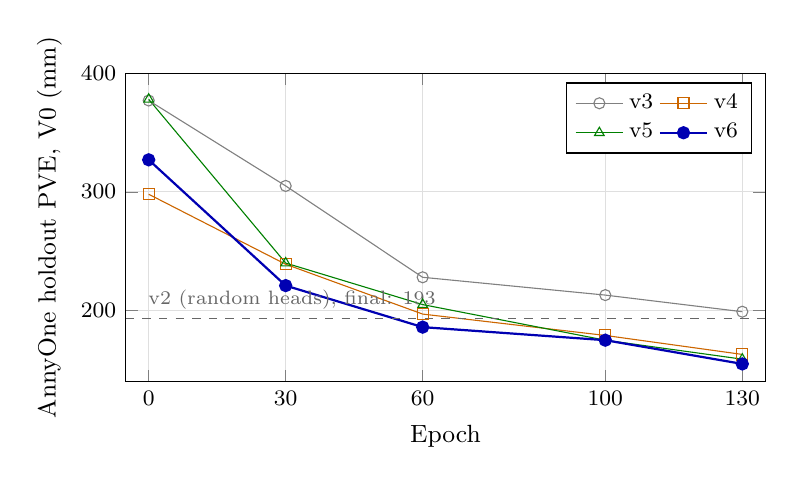
\begin{tikzpicture}
\begin{axis}[
  width=0.8\linewidth, height=5.5cm,
  xlabel={Epoch}, ylabel={AnnyOne holdout PVE, V0 (mm)},
  xmin=-5, xmax=135, ymin=140, ymax=400, xtick={0,30,60,100,130},
  grid=major, grid style={gray!25},
  tick label style={font=\footnotesize}, label style={font=\small},
  legend style={font=\footnotesize, at={(0.98,0.97)}, anchor=north east}, legend columns=2,
]
\addplot[color=gray, mark=o] coordinates {(0,377) (30,305) (60,228) (100,213) (130,199)};
\addlegendentry{v3}
\addplot[color=orange!80!black, mark=square] coordinates {(0,298) (30,239) (60,197) (100,179) (130,163)};
\addlegendentry{v4}
\addplot[color=green!50!black, mark=triangle] coordinates {(0,378) (30,240) (60,205) (100,175) (130,159)};
\addlegendentry{v5}
\addplot[color=blue!70!black, mark=*, thick] coordinates {(0,327) (30,221) (60,186) (100,175) (130,155)};
\addlegendentry{v6}
\draw[dashed, black!60] (axis cs:-5,193) -- (axis cs:135,193) node[pos=0.02, anchor=south west, font=\scriptsize] {v2 (random heads), final: 193};
\end{axis}
\end{tikzpicture}
\caption{Held-out PVE of the ViT-S head-transfer students at equal epochs (setting V0; history, before the depth and
bone fixes and the corrected 3DPW labels). Each student adds one change to the previous one: v4 an HMR-trained
student backbone, v5 a 5-epoch head freeze, v6 projector-fed heads.}
\label{fig:vits-curves}
\end{figure}
